\chapter{单一尺度下的故障诊断模型研究}
\label{cha:chapter2}

\section{引言}

本章主要研究了单一尺度的特征提取方法及故障诊断模型,特征提取过程使用了平均值下采样的方法。
由于下采样的过程中可以指定下采样的核宽度,因此能够得到不同维度的特征向量(即不同尺度
的特征)。本章也通过实验对比研究了特征的不同个数对模型最终的预测精度的影响,从而选择最佳
的特征个数。

本章首先对特征提取过程中用到的实数形式的离散傅立叶变换以及故障诊断模型中用到的支持向量机算法
的基本原理做了简单的介绍,然后详细介绍了本章中设计的单一尺度的特征提取方法,以及基于支持向量
机的级联分类模型,之后简单地介绍了本文各章的实验中都用到的数据集CWRU滚动轴承故障数据集,最后
使用该数据集对本章设计的模型进行了验证。

\section{基本理论}

\subsection{实数形式的傅立叶变换}
\label{subsection:rdft}

离散傅立叶变换(Discrete Fourier Transform, DFT)是信号处理中常用的一种技术,当信号从时域变换到
频域之后,能够将原始信号中包含的信息分为相位和幅度信息,
往往能够更好地反映出信号的频谱结构和变化规律,从而简化信号分析的难度。在信号识别或分
类等应用中,DFT经常被用来提取信号的频域特征。对于具有N个采样点的信号序列$\{x_n\}_{0\leq n < N}$,
它的傅立叶变换如~(\ref{equ:chap2:dft})式所示。
\begin{equation}
\label{equ:chap2:dft}
  \hat{x}_k=\sum_{n=0}^{N-1}x_n e^{-i\frac{2\pi}{N}nk}, k=0,1,...,N-1
\end{equation}

实数形式的离散傅立叶变换(Real Discrete Fourier transform, RDFT)是由Okan Ersoy等人于1985年
提出的一种酉变幻~\cite{ersoy1985real}。RDFT在数据压缩、滤波等很多信号处理应用中的效果比DFT更
加出色~\cite{ersoy1988fast}。同样,RDFT也有类似于快速傅立叶变换
的快速计算方法RFFT~\cite{ersoy1988fast}。同样,对于具有N个采样点的信号序列$\{x_n\}_{0\leq n < N}$,
它的实数形式的傅立叶变换如~(\ref{equ:chap2:rdft})式所示。
\begin{equation}
\label{equ:chap2:rdft}
  \widetilde{x}=
  \begin{cases}
    \left[\hat{x}_0, \text{Re}\hat{x}_1, \text{Im}\hat{x}_1, ..., \text{Re}\hat{x}_{\frac{N}{2}}\right],  & N\text{为偶数}\\
    \left[\hat{x}_0, \text{Re}\hat{x}_1, \text{Im}\hat{x}_1, ..., \text{Im}\hat{x}_{\frac{N-1}{2}}\right],& N\text{为奇数}
  \end{cases}
\end{equation}

本文在信号序列的特征提取阶段使用RDFT而不是DFT的原因如下:

1)实值性

从~(\ref{equ:chap2:dft})式和~(\ref{equ:chap2:rdft})式中可以看出,DFT的结果是一个复数序列,
它的快速计算方法FFT涉及复数加法和乘法。但是在原始信号序列为实数序列时,
RDFT的计算结果仍然是一个实数序列,因此其计算过程完全不需要用到复数的加法和乘法,从而降低了
软硬件实现的复杂性,同时也便于显示和进一步处理。

2)特征个数少

从DFT的定义~(\ref{equ:chap2:dft})式可以看出,DFT的结果具有~(\ref{equ:chap2:symmetry})式所示
的复共轭对称性。
\begin{equation}
\label{equ:chap2:symmetry}
  \hat{x}_n = \hat{x}^*_{N-n}
\end{equation}

因此,在DFT计算所得的序列中,有一半的数据是冗余的,不但增加了计算量,而且会增加随后的分类器
的复杂程度。相反,~(\ref{equ:chap2:rdft})式表示的RDFT在定义的时候就避免了这种冗余,实现起来
更加高效。因此,RDFT在处理很多实信号时,比DFT更加具有优势。

\subsection{支持向量机}

支持向量机是最常用的有监督学习算法之一。在介绍SVM算法之前,首先需要讨论间隔的概念
以及最大间隔分类的思想。接下来会讨论最优间隔分类器以及拉格朗日对偶问题。最后一部分
将介绍使SVM算法能够有效应用于高维特征空间及非线性分类问题的重要技巧:核函数。

\subsubsection{间隔}

在逻辑斯特回归(Logistic Regression)算法中,我们用$h_{\theta}(x) = g(\theta^Tx)$对概率
$p(y = 1|x;\theta)$进行建模。对于输入$x$,当且仅当$h_{\theta}(x) \geq 0.5$
即$\theta^Tx \geq 0$时,预测$y = 1$。对于训练集中的一个正样本(即$y = 1$),$\theta^Tx$
越大,$h_{\theta}(x) = p(y = 1|x;\theta)$也就越大,意味着标签为1的置信度越高。
因此可以得出一个直观的结论,当$\theta^Tx \gg 0$时,预测$y = 1$的置信度是非常高的。
同样地,可以认为在$\theta^Tx \ll 0$时,逻辑斯特回归模型得出的$y = 0$的预测结果也是非常
可信的。给定一个训练集,直观上只要能够找到一个$\theta$使得对任意$y^{(i)} = 1$有
$\theta^Tx^{(i)} \gg 0$并且对任意$y^{(i)} = 0$有$\theta^Tx^{(i)} \ll 0$,那么将会
获得一个非常好的拟合效果。因为在这种情况下,对于所有训练样本,都能得到一个置信度很高
的分类结果。之后会用函数间隔的概念来正式表述这种思想。

下面考虑如图~\ref{fig:margin}所示的二分类问题,图中叉号表示训练集中的正样本,圆圈
表示训练集中的负样本,两类样本之间的直线表示决策边界(也称为分类超平面,由$\theta^Tx = 0$
给出)。
\begin{figure}[ht] % use float package if you want it here
  \centering
  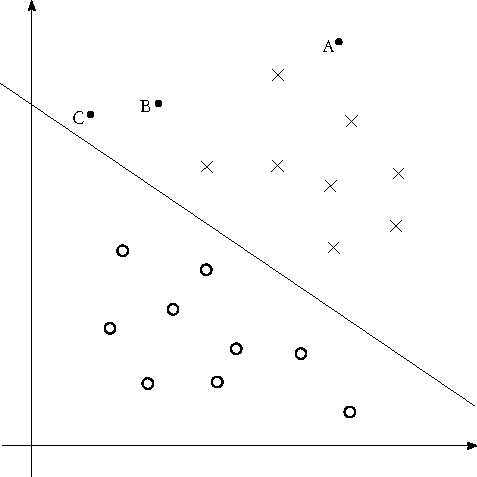
\includegraphics{margin}
  \caption{二分类问题}
  \label{fig:margin}
\end{figure}

从图中可以看到A点离决策边界非常远,如果在A点处对$y$的值进行预测,可以得到一个置信度
非常高的结果$y = 1$。相反,C点离决策边界非常近,虽然根据它在决策边界右侧可以预测得到
$y = 1$,但是即便是决策边界的一个微小的变化都会轻易地导致预测结果变为$y = 0$。也就是说A点
处的预测结果比C点处的预测结果具有更高的置信度,而B点处于这两种情况之间。一般来讲,如果一个点
离分类超平面越远,我们的预测结果的置信度就越高。在给定一个训练集的情况下,我们希望找到一个
决策边界能够对训练集中的所有样本都能做出正确并且置信度高的预测。之后会用几何间隔的概念
来正式表述这种思想。

\subsubsection{符号定义}

为了表述方便,首先需要引入一种新的记法来讨论分类问题。重新明确一下要解决的问题:特征为
$x$,标签为$y$的二分类问题,求一个线性分类器。从现在开始,使用$y \in \{-1, 1\}$(而不是
$\{0, 1\}$)来表示类别标签。另外,用参数$w, b$(而不是$\theta$)来表示线性分类器,
如~(\ref{equ:chap2:classifier})式所示。
\begin{equation}
  \label{equ:chap2:classifier}
  h_{w,b}(x) = g(w^Tx+b)
\end{equation}

此处如果$z \geq 0$那么$g(z) = 1$,否则$g(z) = -1$。

\subsubsection{函数间隔和几何间隔}

下面正式给出函数间隔和几何间隔的定义。给定一个训练样本$(x^{(i)},y^{(i)})$,定义$(w,b)$相对
于训练样本的函数间隔如~(\ref{equ:chap2:fmargin_i})式所示。
\begin{equation}
  \label{equ:chap2:fmargin_i}
  \hat{\gamma}^{(i)} = y^{(i)}(w^Tx+b)
\end{equation}

从~(\ref{equ:chap2:fmargin_i})式可以看出,在$y^{(i)} = 1$时,为了使函数间隔尽量大(即预测结果
置信度尽量高),需要使$w^Tx+b$为一个尽可能大的正数。相反,在$y^{(i)} = -1$时,为了
使函数间隔尽量大,$w^Tx+b$需要为一个尽可能小的负数。此外,$y^{(i)}(w^Tx+b) > 0$意味着
预测结果是正确的。因此,大的函数间隔代表了准确且高置信度的预测结果。

给定一个训练集$S = \{(x^{(i)},y^{(i)});i = 1, ..., m\}$,定义$(w,b)$关于$S$的函数边界为
所有训练样本的函数边界的最小值,记为$\hat{\gamma}$,可以用~(\ref{equ:chap2:fmargin})式表示。
\begin{equation}
  \label{equ:chap2:fmargin}
  \hat{\gamma} = \min_{i=1,...,m}\hat{\gamma}^{(i)}
\end{equation}

对于这样一个线性分类器,如果用$2w$和$2b$分别替换$w$和$b$,那么$g(w^Tx+b)=g(2w^Tx+2b)$,$h_{w,b}(x)$
将保持不变。也就是说$g$和$h_{w,b}(x)$仅仅取决于$w^Tx+b$的符号而不是大小。然而将$(w,b)$替换为
$(2w,2b)$会导致函数间隔变为原来的两倍。因此,需要引入一些归一化条件,比如令$\|w\|=1$。

下面讨论几何边界。考虑图~\ref{fig:margin2}所示的分类问题:
\begin{figure}[ht] % use float package if you want it here
  \centering
  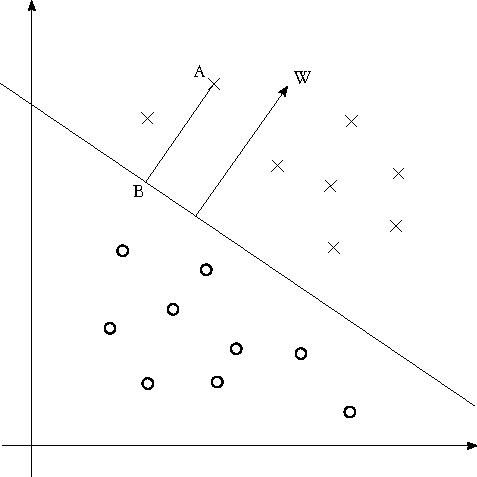
\includegraphics{margin2}
  \caption{几何间隔}
  \label{fig:margin2}
\end{figure}

图中画出了与$(w,b)$所对应的决策边界,以及向量$w$。显然,$w$是垂直于分类超平面的。A点是某个
训练样本的输入$x^{(i)}$,其标签为$y^{(i)} = 1$,到决策边界的距离$\gamma^{(i)}$由线段AB给出。

下面来计算$\gamma^{(i)}$的值。由于$w/\|w\|$是一个与$w$同方向的单位向量,并且A点坐标为$x^{(i)}$,
因此可以得到B点的坐标为$x^{(i)} - \gamma^{(i)} \cdot w/\|w\|$。进一步由于B点在决策边界上,
而所有决策边界上的点$x$均满足$w^Tx+b=0$,因此得到:
\begin{equation}
  \label{equ:chap2:gmargin_i_1}
  w^T\left(x^{(i)} - \gamma^{(i)}\frac{w}{\|w\|}\right) + b = 0
\end{equation}

解得:
\begin{equation}
  \label{equ:chap2:gmargin_i_2}
  \gamma^{(i)} = \frac{w^Tx^{(i)}+b}{\|w\|} = \left(\frac{w}{\|w\|}\right)^Tx^{(i)} + \frac{b}{\|w\|}
\end{equation}

~(\ref{equ:chap2:gmargin_i_2})式对任意正样本(即$y^{(i)} = 1$)成立。对于一般情况,
定义$(w,b)$关于训练样本$(x^{(i)}, y^{(i)})$的几何间隔为:
\begin{equation}
  \label{equ:chap2:gmargin_i_3}
  \gamma^{(i)} = y^{(i)}\left(\left(\frac{w}{\|w\|}\right)^Tx^{(i)} + \frac{b}{\|w\|}\right)
\end{equation}

从~(\ref{equ:chap2:gmargin_i_3})式可以看出,如果$\|w\|=1$,那么函数间隔将等于几何间隔。可以看出
与函数间隔不同的是如果用$2w$和$2b$分别替换$w$和$b$,那么几何间隔将不会发生改变。也正是由于
几何间隔相对于参数缩放的这种不变性,当我们使用训练数据来拟合$w$和$b$的时候,可以引入任意
的缩放约束,而不会改变模型本身。比如,可以令$\|w\|=1$,或者$|w_1|=5$,或者$|w_1+b|+|w_2|=2$等。

同样,给定一个训练集$S=\{(x^{(i)},y^{(i)});i=1,...,m\}$,定义$(w,b)$关于$S$的几何间隔
为所有训练样本的几何间隔的最小值,如~(\ref{equ:chap2:gmargin})式所示。
\begin{equation}
  \label{equ:chap2:gmargin}
  \gamma=\min_{i=1,...,m}\gamma^{(i)}
\end{equation}

\subsubsection{最优间隔分类器}

给定一个训练集,从前面的讨论可以得到一个自然的结论:通过寻找最大化几何间隔的决策边界,就能得到
一个在训练集上拟合得很好的分类器。假设训练集上的两类样本是线性可分的,即存在分类超平面可以完全
将两类样本分开,那么寻找最大化几何间隔的超平面的问题可以表述为~(\ref{equ:chap2:opt1})式所示的优化
问题。
\begin{equation}
  \label{equ:chap2:opt1}
  \begin{aligned}
    \max_{\gamma,w,b} &
    & & \gamma \\
    \text{s.t.} &
    & & y^{(i)}\left(w^Tx^{(i)}+b\right)\geq \gamma, i=1,...,m \\
    \quad &
    & & \|w\|=1
  \end{aligned}
\end{equation}

即最大化$\gamma$,使得每个训练样本的函数间隔都至少是$\gamma$。约束条件$\|w\|=1$保证了函数间隔和
几何间隔相等,从而保证了所有训练样本的几何间隔也至少是$\gamma$。

由于约束条件$\|w\|=1$是非凸的,因此这个问题不易直接用标准优化软件工具求解。因此将其转化为
~(\ref{equ:chap2:opt2})式所示的优化问题。
\begin{equation}
  \label{equ:chap2:opt2}
  \begin{aligned}
    \max_{\hat{\gamma},w,b} &
    & & \frac{\hat{\gamma}}{\|w\|} \\
    \text{s.t.} &
    & & y^{(i)}\left(w^Tx^{(i)}+b\right)\geq \hat{\gamma}, i=1,...,m
  \end{aligned}
\end{equation}

由于几何间隔和函数间隔之间存在关系$\gamma=\hat{\gamma}/\|w\|$,因此我们最大化$\hat{\gamma}/\|w\|$,
使得所有训练样本的函数间隔至少为$\hat{\gamma}$。这样虽然去掉了约束条件$\|w\|=1$,但是引入了非凸
的目标函数$\frac{\hat{\gamma}}{\|w\|}$。

前面提到可以在$w$和$b$上增加任意一个缩放约束条件而不改变问题本身。因此可以令$w,b$关于训练集
的函数间隔等于1。
\begin{equation}
  \label{equ:chap2:constrain}
  \hat{\gamma} = 1
\end{equation}

将~(\ref{equ:chap2:constrain})式代入~(\ref{equ:chap2:opt2}),并将最大化$\hat{\gamma}/\|w\|=1/\|w\|$
替换为最小化$\frac{1}{2}\|w\|^2$,可以得到~(\ref{equ:chap2:opt3})式所示的优化问题。
\begin{equation}
  \label{equ:chap2:opt3}
  \begin{aligned}
    \min_{w,b} &
    & & \frac{1}{2}\|w\|^2 \\
    \text{s.t.} &
    & & y^{(i)}\left(w^Tx^{(i)}+b\right)\geq 1, i=1,...,m
  \end{aligned}
\end{equation}

\subsubsection{拉格朗日对偶问题}

虽然~(\ref{equ:chap2:opt3})式表示的优化问题可以使用商业的二次规划(Quadratic Programming, QP)
代码来求解,但是一般情况下都是选择将其转化为拉格朗日对偶形式来求解。这对使用核函数来
使模型更好地应用于高维特征空间是至关重要的。另外,其对偶形式可以通过一些迭代算法来求解,
通常情况下比直接使用QP软件求解更加高效。

~(\ref{equ:chap2:opt3})式表示的原问题对应的拉格朗日函数如~(\ref{equ:chap2:lagrangian})式所示。
\begin{equation}
  \label{equ:chap2:lagrangian}
  \mathcal{L}(w,b,\alpha)=\frac{1}{2}\|w\|^2-\sum_{i=1}^m \alpha_i\left[y^{(i)}\left(w^Tx^{(i)}+b\right)-1\right]
\end{equation}

固定$\alpha$,最小化$\mathcal{L}(w,b,\alpha)$,即$\mathcal{L}$关于$w$和$b$的偏导数为0:
\begin{equation}
  \label{equ:chap2:derivative_w}
  \nabla_w\mathcal{L}(w,b,\alpha)=w-\sum_{i=1}^{m}\alpha_iy^{(i)}x^{(i)}=0
\end{equation}

解得:
\begin{equation}
  \label{equ:chap2:expression_w}
  w=\sum_{i=1}^{m}\alpha_iy^{(i)}x^{(i)}
\end{equation}

$\mathcal{L}$关于$b$的偏导数为0,得到:
\begin{equation}
  \label{equ:chap2:derivative_b}
  \frac{\partial}{\partial b}\mathcal{L}(w,b,\alpha)=\sum_{i=1}^m\alpha_iy^{(i)}=0
\end{equation}

将~(\ref{equ:chap2:expression_w})式和~(\ref{equ:chap2:derivative_b})式代入~(\ref{equ:chap2:lagrangian})式
化简可得:
\begin{equation}
  \label{equ:chap2:dual_objective}
  \mathcal{L}(w,b,\alpha)=\sum_{i=1}^m\alpha_i-\frac{1}{2}\sum_{i,j=1}^m
  y^{(i)}y^{(j)}\alpha_i\alpha_j(x^{(i)})^Tx^{(j)}
\end{equation}

加上拉格朗日乘子$\alpha_i$非负的约束条件,以及~(\ref{equ:chap2:derivative_b})式的约束条件,可以得到
对偶优化问题如~(\ref{equ:chap2:dual_opt})式所示。
\begin{equation}
  \label{equ:chap2:dual_opt}
  \begin{aligned}
    \max_{\alpha} &
    & & \sum_{i=1}^m\alpha_i-\frac{1}{2}\sum_{i,j=1}^m
    y^{(i)}y^{(j)}\alpha_i\alpha_j\langle x^{(i)},x^{(j)}\rangle\\
    \text{s.t.} &
    & & \alpha_i\geq 0, i=1,...,m \\
    \quad &
    & & \sum_{i=1}^m\alpha_iy^{(i)}=0
  \end{aligned}
\end{equation}

针对这个优化问题,已经有很多基于迭代的算法被设计出来,其中最经典的是序贯最小优化算法
(SMO, Sequential Minimal Optimization)~\cite{platt1998sequential},
很多其他算法都是基于该算法设计的。这些算法使得我们不必直接通过二次规划的方式求解该优化问题,
保证了模型在特征维度很大或者样本数量很多的情况下仍然能够有效求解。

当获得对偶问题的最优解$\alpha^*$之后,可以通过~(\ref{equ:chap2:expression_w})式来计算$w^*$,
并通过~(\ref{equ:chap2:expression_b})式来计算$b^*$。
\begin{equation}
  \label{equ:chap2:expression_b}
  b^*=-\frac{\max_{i:y^{(i)}=-1}{w^*}^Tx^{(i)}+\min_{i:y^{(i)}=1}{w^*}^Tx^{(i)}}{2}
\end{equation}

最后,可以通过计算${w^*}^Tx+b^*$的值来对样本$x$的标签进行预测,如果该值大于0,那么将预测$y=1$,
反之则预测$y=-1$。

\subsubsection{不可分的情况及正则化}

在前面推导SVM模型的时候都假定数据是线性可分的,但是并不能保证事实情况总是如此。
此外,即便是能够找到这样一个分类超平面, 也不一定是就是我们想要的结果,
因为这样的分类超平面可能是受到了一些异常点的干扰。举个例子,
图~\ref{fig:margin3}显示了一个最优分类超平面,当一个异常点被加入到左上角区域时
(如~\ref{fig:margin4}所示),分类超平面产生一个非常大的变动,导致分类器的间隔急剧减小。
\begin{figure}[ht]
  \centering%
  \subcaptionbox{正常情况下的决策面\label{fig:margin3}} %标题的长度,超过则会换行,如下一个小图。
  {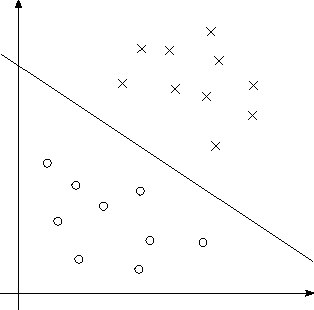
\includegraphics{margin3}}%
  \hspace{6em}%
  \subcaptionbox{有异常点时的决策面\label{fig:margin4}}
  {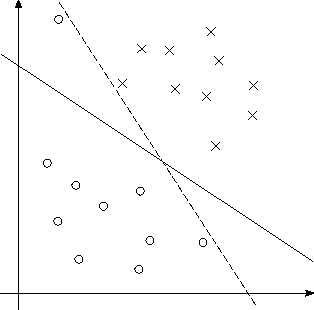
\includegraphics{margin4}}
  \caption{决策面受异常点干扰示例}
  \label{fig:margin3+4}
\end{figure}

为了使得模型在非线性可分的情况下仍然有效,同时对异常点的干扰更加鲁棒,将原来的优化问题
重新写为~(\ref{equ:chap2:opt_reg})式:
\begin{equation}
  \label{equ:chap2:opt_reg}
  \begin{aligned}
    \min{w,b} &
    & & \frac{1}{2}\|w\|^2+C\sum_{i=1}^m\xi_i \\
    \text{s.t.} &
    & & y^{(i)}\left(w^Tx^{(i)}+b\right)\geq 1-\xi_i, i=1,...,m \\
    \quad &
    & & \xi_i \geq 0, i=1,...,m
  \end{aligned}
\end{equation}

即允许样本的函数间隔小于1(等价于被错分),并且在目标函数中引入一个惩罚项$C\xi_i$。参数C
控制惩罚项所占的权重,被称为惩罚因子。同样地,可以得到该优化问题的拉格朗日对偶问题,如
~(\ref{equ:chap2:dual_opt_reg})所示。
\begin{equation}
  \label{equ:chap2:dual_opt_reg}
  \begin{aligned}
    \max_{\alpha} &
    & & \sum_{i=1}^m\alpha_i-\frac{1}{2}\sum_{i,j=1}^m
    y^{(i)}y^{(j)}\alpha_i\alpha_j\langle x^{(i)},x^{(j)}\rangle\\
    \text{s.t.} &
    & & 0\leq\alpha_i\leq C, i=1,...,m \\
    \quad &
    & & \sum_{i=1}^m\alpha_iy^{(i)}=0
  \end{aligned}
\end{equation}

\subsubsection{核函数}

从~(\ref{equ:chap2:dual_opt_reg})中可以看出,模型可以写成一个完全关于内积$\langle x,z\rangle$的形式,
意味着如果使用一种特征映射$\phi$将输入特征$x$变换到空间$\phi(x)$,那么可以将所有的内积
替换为$\langle\phi(x),\phi(z)\rangle$。一般地,给定一种特征映射$\phi$,定义与之对应的核函数如
~(\ref{equ:chap2:kernel})所示。
\begin{equation}
  \label{equ:chap2:kernel}
  K(x,z)=\phi(x)^T\phi(z)
\end{equation}

特别地,当$\phi(x)=x$时,$K(x,z)=\langle x,z\rangle$,称之为线性核,此时模型即为
~(\ref{equ:chap2:dual_opt_reg})式所示。除此之外,还有很多常用的核函数,举例如下:

1)多项式核函数
\begin{equation}
  \label{equ:chap2:polynomial_kernel}
  K(x,z)=(x^Tz+c)^d
\end{equation}

2)高斯核函数
\begin{equation}
  \label{equ:chap2:gauss_kernel}
  K(x,z)=\exp\left(-\frac{\|x-z\|^2}{2\sigma^2}\right)
\end{equation}

3)sigmoid核函数
\begin{equation}
  \label{equ:chap2:sigmoid_kernel}
  K(x,z)=\tanh(\alpha x^Tz+c)
\end{equation}

\section{基于支持向量机的级联故障诊断模型}

\subsection{基于下采样的单一尺度特征提取方法}

给定一个信号片段$x$,其采样点个数为$N$,即$x=(x_1,x_2,...,x_N)^T$。首先
对$x$进行~(\ref{equ:chap2:rdft})式所示的实数形式的离散傅立叶变换,得到RDFT
频谱序列$\widetilde{x}$,由~\ref{subsection:rdft}节中的介绍可知,$\widetilde{x}$
的维度也是$N$,即$\widetilde{x} = (\widetilde{x}_1, \widetilde{x}_2, ...,
\widetilde{x}_N)^T$。为了避免样本间相位不同对最终模型的诊断精度产生影响,同
时也为了避免在后续的操作中正负值之间相互抵消,本文对RDFT频谱序列取了绝对值,
即$X = (|\widetilde{x}_1|, |\widetilde{x}_2|, ..., |\widetilde{x}_N|)^T$,本
文中之后提到的频谱序列均是指$X$。接下来使用核宽度为$F$的平均值下采样来进
一步提取特征,假设我们希望得到的特征个数为$L$,那么$F$和$L$满足~(\ref{equ:chap2:f_l})
式所示的关系。
\begin{equation}
  \label{equ:chap2:f_l}
  F=\lfloor N/L \rfloor
\end{equation}

其中$\lfloor x \rfloor$表示不大于$x$的最大整数。将序列$X$等分为$L$个连续不重
叠的小区间,并且对各个区间内的值进行平均,得到长度为L的特征向量$V=(V_1,V_2,...,V_L)^T$。
这个过程可以用~(\ref{equ:chap2:pooling})式表示。
\begin{equation}
  \label{equ:chap2:pooling}
  V_k=\frac{1}{F}\sum_{j=1}^{F}X_{(k-1)F+j}, k=1,2,...,L
\end{equation}

使用这样一种特征提取过程的优势在于,相对于直接使用信号频谱序列作为输入特征,
可以在保证其整体分布趋势近似不变的同时,大幅度地降低特征向量的维度,
从而提升分类器训练和预测过程的速度,保证诊断过程的是实时性。此外,在特征提取阶段
使用平均值下采样还可以降低某些特定频段的噪声所带来的影响,使得整个模型具有更好的
鲁棒性。此外,在使用平均值下采样的过程中,设定了一个参数$L$,也就是最终得到的
特征个数,本文会在之后的实验中对比该参数的变化对模型的影响,从而选择最佳的参数值。

图~\ref{fig:average_pooling}显示了一个采样点数为384的信号片段,其对应的频谱序列,
以及使用平均值下采样提取的特征个数为32的特征向量。
\begin{figure}[ht] % use float package if you want it here
  \centering
  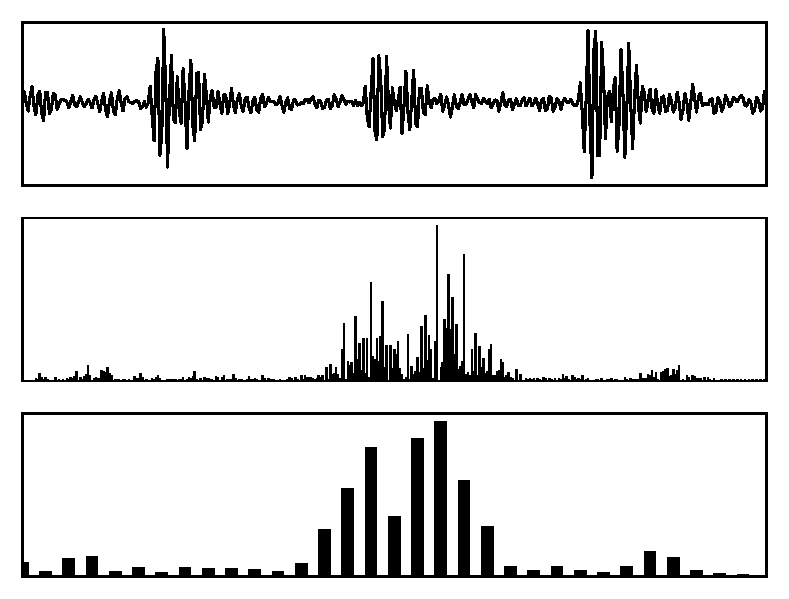
\includegraphics[height=8cm]{average_pooling}
  \caption{原始信号片段,RDFT频谱和特征向量}
  \label{fig:average_pooling}
\end{figure}

\subsection{分类模型}
\label{subsection:cascade_model}

虽然可以将提取到的特征向量直接输入到一个多分类模型中进行训练,就可以完成故障分类
的任务,但是在某些特定的情况下,尤其是当数据的类别标签具有明显的层次性(比如在故障诊断
问题当中,最常见的就是存在多种不同的故障位置,并且每一类故障位置可能会进一步有不同的
故障尺寸等等)的时候,设计一个由多个子分类器构成的级联分类器往往会更加有效。

假设在一个故障诊断问题中,存在三类可能的故障位置,记为位置A、位置B、位置C,
每一类故障位置都可能会发生3种不同程度的故障,记为尺寸1、尺寸2、尺寸3,同时还有一类
是正常样本。那么可以针对故障类别的这种层次性,设计一个由5个子分类器构成的级联分类
过程,如图~\ref{fig:cascade_classifier}所示。
\begin{figure}[ht] % use float package if you want it here
  \centering
  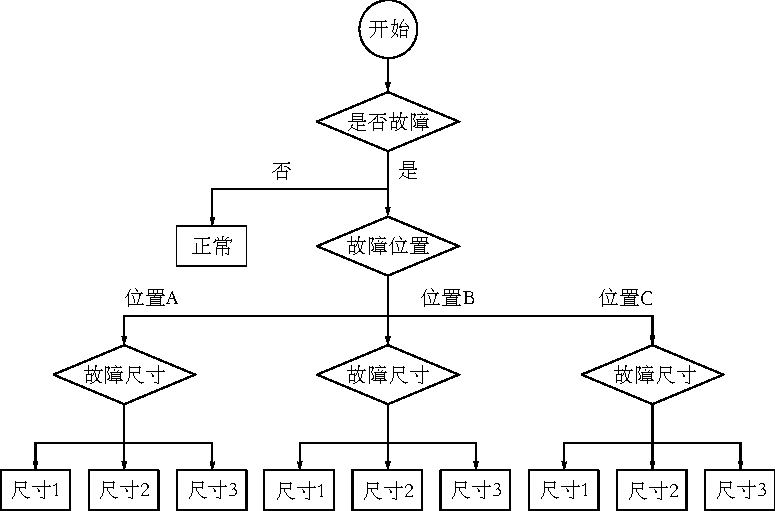
\includegraphics[height=9cm]{cascade_classifier}
  \caption{级联分类过程示意图}
  \label{fig:cascade_classifier}
\end{figure}

图中每个菱形表示一个子分类器,可以根据实际情况采用不同的算法实现,不同子分类器所用的
算法也不一定相同。图中的每一个矩形框代表一种故障类型,可以看出这个例子中总共有10类样本,
其中一类是正常样本。可以看出,整个级联分类过程整体上分为三个阶段,第一个阶段由一个子分
类器判断是否为故障样本;接下来一个阶段由一个子分类器判断故障发生的位置;最后一个阶段
用三个子分类器分别判断故障的尺寸。

\section{实验验证}

\subsection{实验数据}

本文的所有实验所用的数据均是来自凯斯西储大学(Case Western Reserve University, CWRU)
的滚动轴承加速度测量数据,其中包括正常工作下的轴承数据和在各种不同故障位置和故障
尺寸下的轴承数据。在旋转机械故障诊断领域,该数据集已经成为标准的测试数据集之一,已经有很多
研究人员使用该数据集来验证其故障诊断模型。

数据采集的实验装置如图~\ref{fig:teststand}所示,测试台由一个2马力的三相感应电机(左)、
扭矩传感器和编码器(中间)、测力计(右)和控制电子设备(图中未显示)组成。 
用来收集振动数据的加速度传感器被磁性底座固定在轴承上方的机壳上,处于电机外壳的驱动端和
风扇端的12点钟位置。实验中使用16通道DAT记录仪收集振动信号,并在Matlab环境中进行后续处理。
所有数据文件均采用Matlab(*.mat)格式保存。该数据集以12kHz的采样频率收集和记录数据,另外
也采集了采样频率为48kHz时的数据,用于驱动端的轴承故障研究。
\begin{figure}[ht]
  \centering
  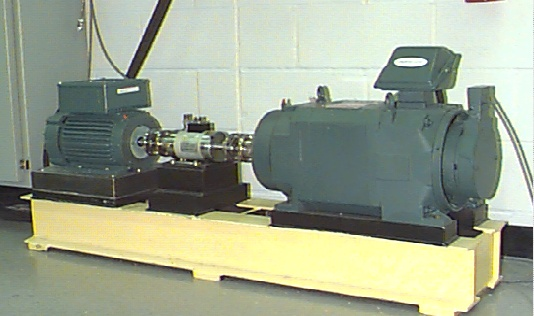
\includegraphics[height=6cm]{teststand}
  \caption{滚动轴承振动数据采集实验台}
  \label{fig:teststand}
\end{figure}

数据采集的实验过程中所用的轴承包括两种,一种是型号为6205-2RS JEM的SKF深沟型轴承,
另一种是型号为6203-2RS JEM的SKF深沟型轴承,表~\ref{tab:bearing_params}列出了型号为
6205-2RS JEM的SKF深沟型轴承的一些主要的几何参数。
\begin{table}[htb]
  \centering
  \begin{minipage}[t]{0.8\linewidth}
  \caption{6205-2RS JEM SKF深沟型轴承几何参数}
  \label{tab:bearing_params}
    \begin{tabularx}{\linewidth}{lXXXXX}
      \toprule[1.5pt]
      滚珠个数 & 内圈直径(英寸)& 外圈直径(英寸)& 轴承厚度(英寸)& 滚珠直径(英寸)& 轴承节径(英寸) \\\midrule[1pt]
      9 & 0.9843 & 2.0472 & 0.5906 & 0.3126 & 1.537 \\\bottomrule[1.5pt]
    \end{tabularx}
  \end{minipage}
\end{table}

轴承的状态除了正常之外,还有内圈故障、钢球故障和外圈故障三种类型,使用火花放电
的方法在测试轴承上引入7密耳、14密耳、21密耳、28密耳(1密尔等于0.001英寸)四种不
同损伤直径的单点故障。电机的负载可以通过风机来调节,可以产生0-3马力的载荷,从而
可以研究不同负载情况下轴承的故障特征。

为了验证本文在各章节中设计的故障诊断模型对故障位置及故障尺寸的识别能力,本文选取
了在采样频率为12kHz,负载为0马力情况下的12种不同类别的轴承振动数据,对所设计的模
型进行训练和测试。由于CWRU数据集中每一种类别的数据都存储在一个Matlab文件(*.mat)
中,每一个文件都对应一个至少包含12000个连续采样点的原始信号。因此,为了获得足够数
量的样本对设计的故障诊断模型进行训练和预测,本文从每个原始信号中随机地截取M个长度
为N的信号片段,并且将其中的$3M/4$个信号片段作为训练样本,其余$M/4$个信号片段作为
预测样本。在选择$N$值的时候,一方面要保证能够从有限的采样点中截取到足够多的信号片
段来训练模型,因此$N$值不能太大;另一方面要保证截取的长度为N的信号片段中能够包含
足够的信息,因此N值也不能太小。在本文的所有实验中均使用$N=384$。此外,M的大小根据
原始信号的长度来确定,不同故障类别的数据包含的信号片段个数M略有不同。这12类样本对
应的故障位置、故障尺寸以及样本个数如表~\ref{tab:class_desc}所示。
\begin{table}[htb]
  \centering
  \begin{minipage}[t]{0.7\linewidth} % 如果想在表格中使用脚注,minipage是个不错的办法
  \caption{12类数据对应的故障位置和尺寸}
  \label{tab:class_desc}
    \begin{tabularx}{\linewidth}{XXXX}
      \toprule[1.5pt]
      类别标签 & 故障位置 & 故障尺寸 & 样本个数 \\
      \midrule[1pt]
      0  & 无   & 无    & 1579 \\
      \midrule[1pt]
      1  & 钢球 & 0.007 &  710 \\
      2  & 钢球 & 0.014 &  784 \\
      3  & 钢球 & 0.021 &  785 \\
      4  & 钢球 & 0.028 &  777 \\
      \midrule[1pt]
      5  & 内圈 & 0.007 &  780 \\
      6  & 内圈 & 0.014 &  784 \\
      7  & 内圈 & 0.021 &  786 \\
      8  & 内圈 & 0.028 &  777 \\
      \midrule[1pt]
      9  & 外圈 & 0.007 &  785 \\
      10 & 外圈 & 0.014 &  784 \\
      11 & 外圈 & 0.021 &  788 \\
      \bottomrule[1.5pt]
    \end{tabularx}
  \end{minipage}
\end{table}

图~\ref{fig:series}展示了这12类轴承振动数据,图中从左至右,从上到下
依次对应类别标签为0-11的数据。每一类数据都随机地显示了3个样本。
\begin{figure}[ht]
  \centering
  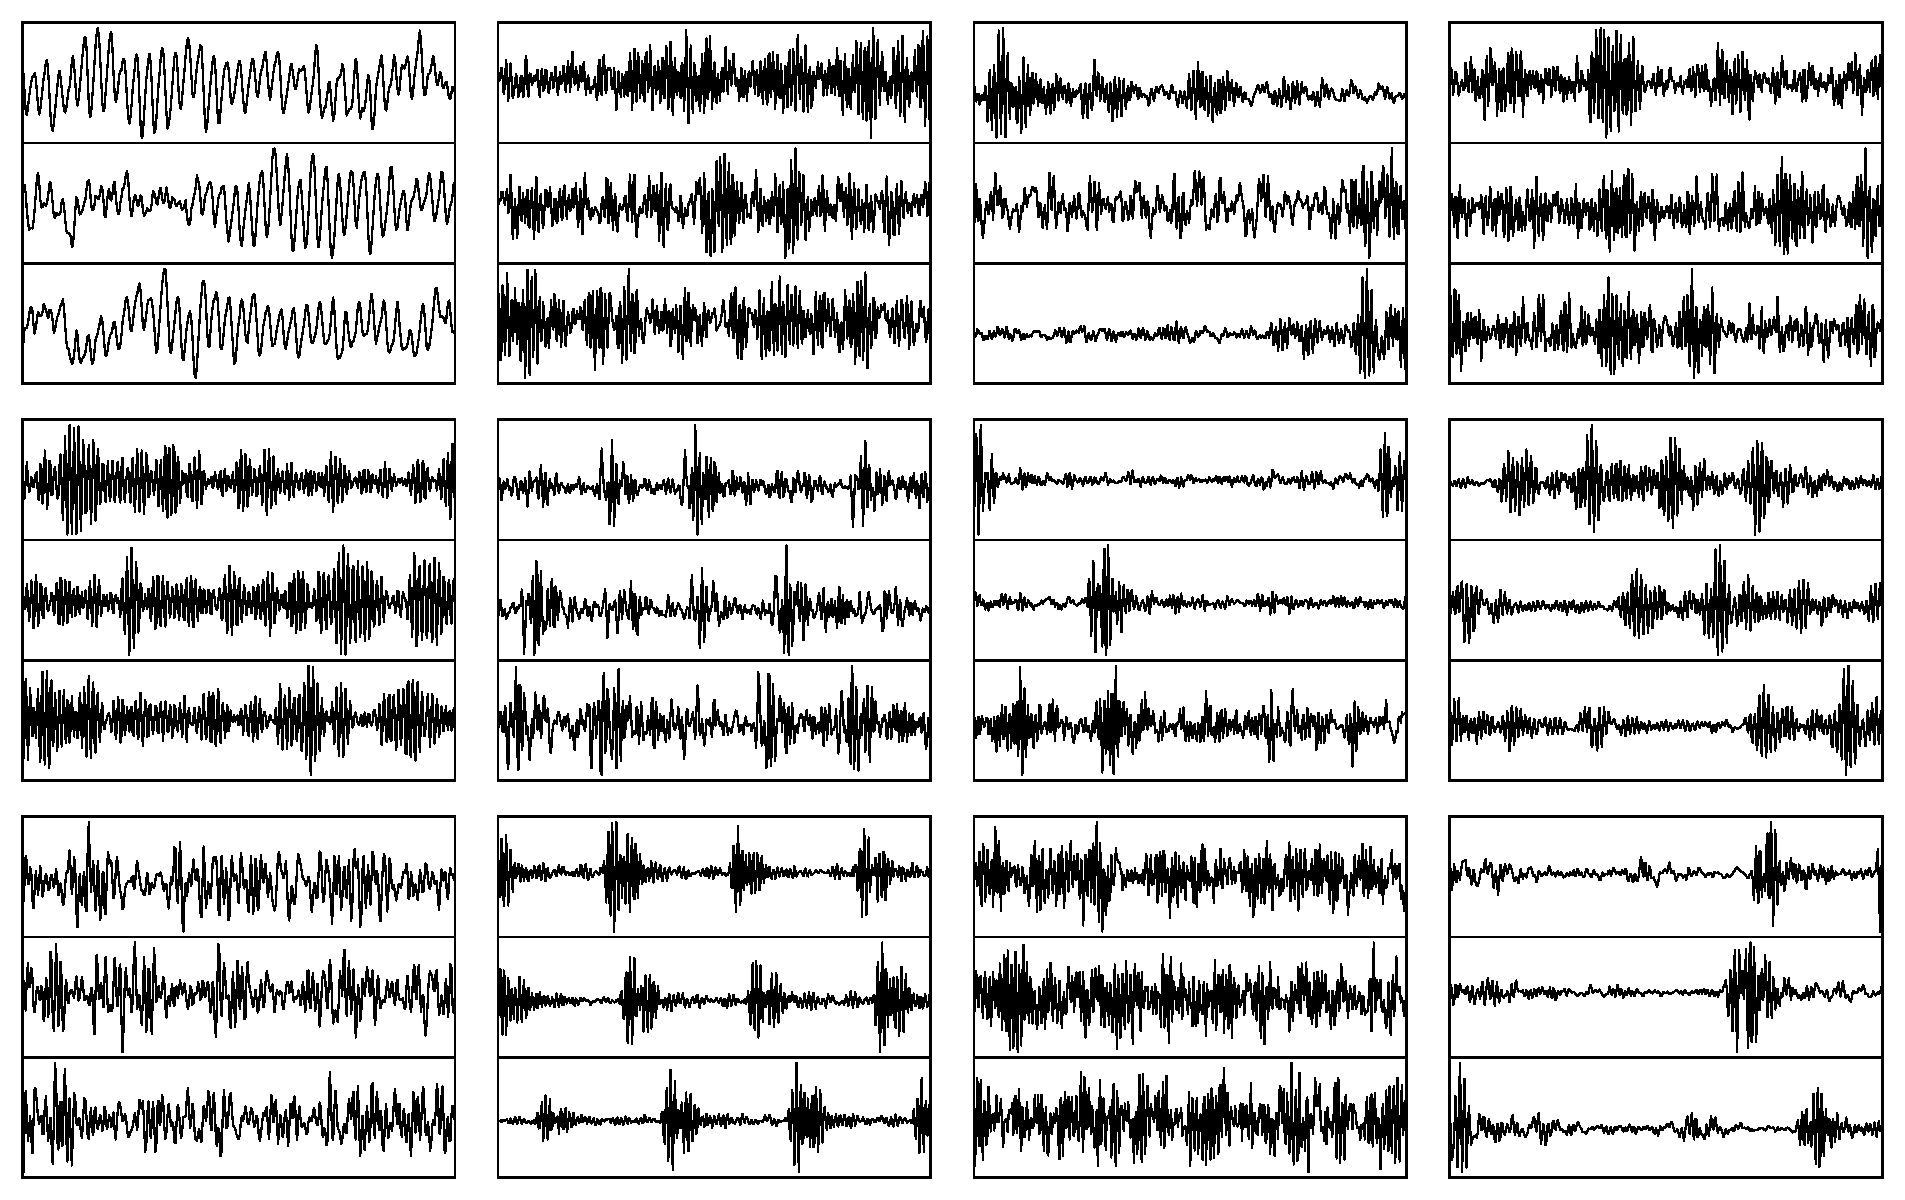
\includegraphics[height=8cm]{series}
  \caption{12类信号片段波形}
  \label{fig:series}
\end{figure}

\subsection{实验过程}

从表~\ref{tab:class_desc}中可以看到,这12类数据中包含一类正常状态,3种不同尺
寸的外圈故障,以及4种不同尺寸的钢球和内圈故障。根据~\ref{subsection:cascade_model}
节中设计的级联分类方法,以及本文使用的这12类数据类别间明显的层次性,本文设计了如图~\ref{fig:cascade_classifier_exp}
所示的级联故障诊断模型,分类器输出的类别标签与实际样本的对应关系参见表~\ref{tab:class_desc}。
\begin{figure}[ht]
  \centering
  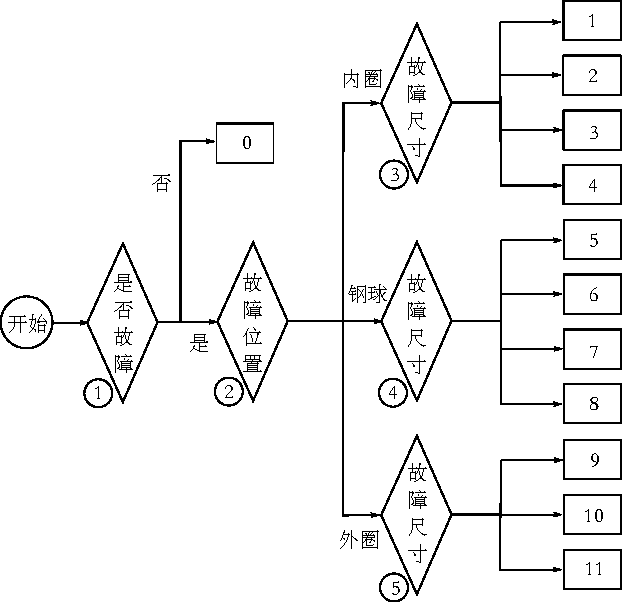
\includegraphics[height=11cm]{cascade_classifier_exp}
  \caption{CWRU数据级联分类模型}
  \label{fig:cascade_classifier_exp}
\end{figure}

在这个级联故障诊断模型中总共有5个子分类器,图~\ref{fig:cascade_classifier_exp}
中将这5个子分类器分别编号为1 - 5。1号子分类器是一个二分类器,用于判断一
个样本是否为故障样本,使用全部12类样本进行训练;2号子分类器输出3种故障
位置,使用除正常样本之外的11类样本进行训练;3、4、5号子分类器分别输出4、
4、3种故障尺寸,训练期间分别使用各自故障位置的4、4、3类不同故障尺寸的样
本。图中各个子分类器输出标签个数、训练过程中用到的数据,以及各个子分类
器的功能如表~\ref{tab:classifier_desc}所示,其中12类数据的标签对应的故
障情况参见表~\ref{tab:class_desc}。
\begin{table}[htb]
  \centering
  \begin{minipage}[t]{0.8\linewidth}
  \caption{各子分类器详细说明}
  \label{tab:classifier_desc}
    \begin{tabularx}{\linewidth}{lXXX}
      \toprule[1.5pt]
      分类器序号 & 分类个数 & 训练所用数据 & 功能 \\\midrule[1pt]
      1 & 2 & 0-11 & 判断是否故障\\
      2 & 3 & 1-11 & 判断故障位置\\
      3 & 4 & 1-4 & 判断钢球故障尺寸\\
      4 & 4 & 5-8 & 判断内圈故障尺寸\\
      5 & 3 & 9-11 & 判断外圈故障尺寸\\
      \bottomrule[1.5pt]
    \end{tabularx}
  \end{minipage}
\end{table}

每个子分类器均使用了SVM算法,选用径向基函数(Radial Basis Function, RBF)
作为SVM的核函数,核函数系数设定为$1/N$。以信号片段的RDFT频谱作为SVM算法
的输入,并且各子分类器之间单独进行训练,最后在预测阶段按照图~\ref{fig:cascade_classifier_exp}
中的级联过程逐步进行预测,得到最终的预测标签。

\subsection{实验结果及分析}
\label{subsection:cascade_result}

由于通过随机截取来生成样本的过程会导致同一类样本间存在很大的相位差别,
因此直接使用信号片段来训练分类器的效果会比较差。因此,我们使用RDFT对
信号片段做预处理,得到对应的频谱序列$X$,图~\ref{fig:series}中展示的
$12\times 3$个信号片段对应的RDFT频谱序列如图~\ref{fig:rdft}所示。
\begin{figure}[ht]
  \centering
  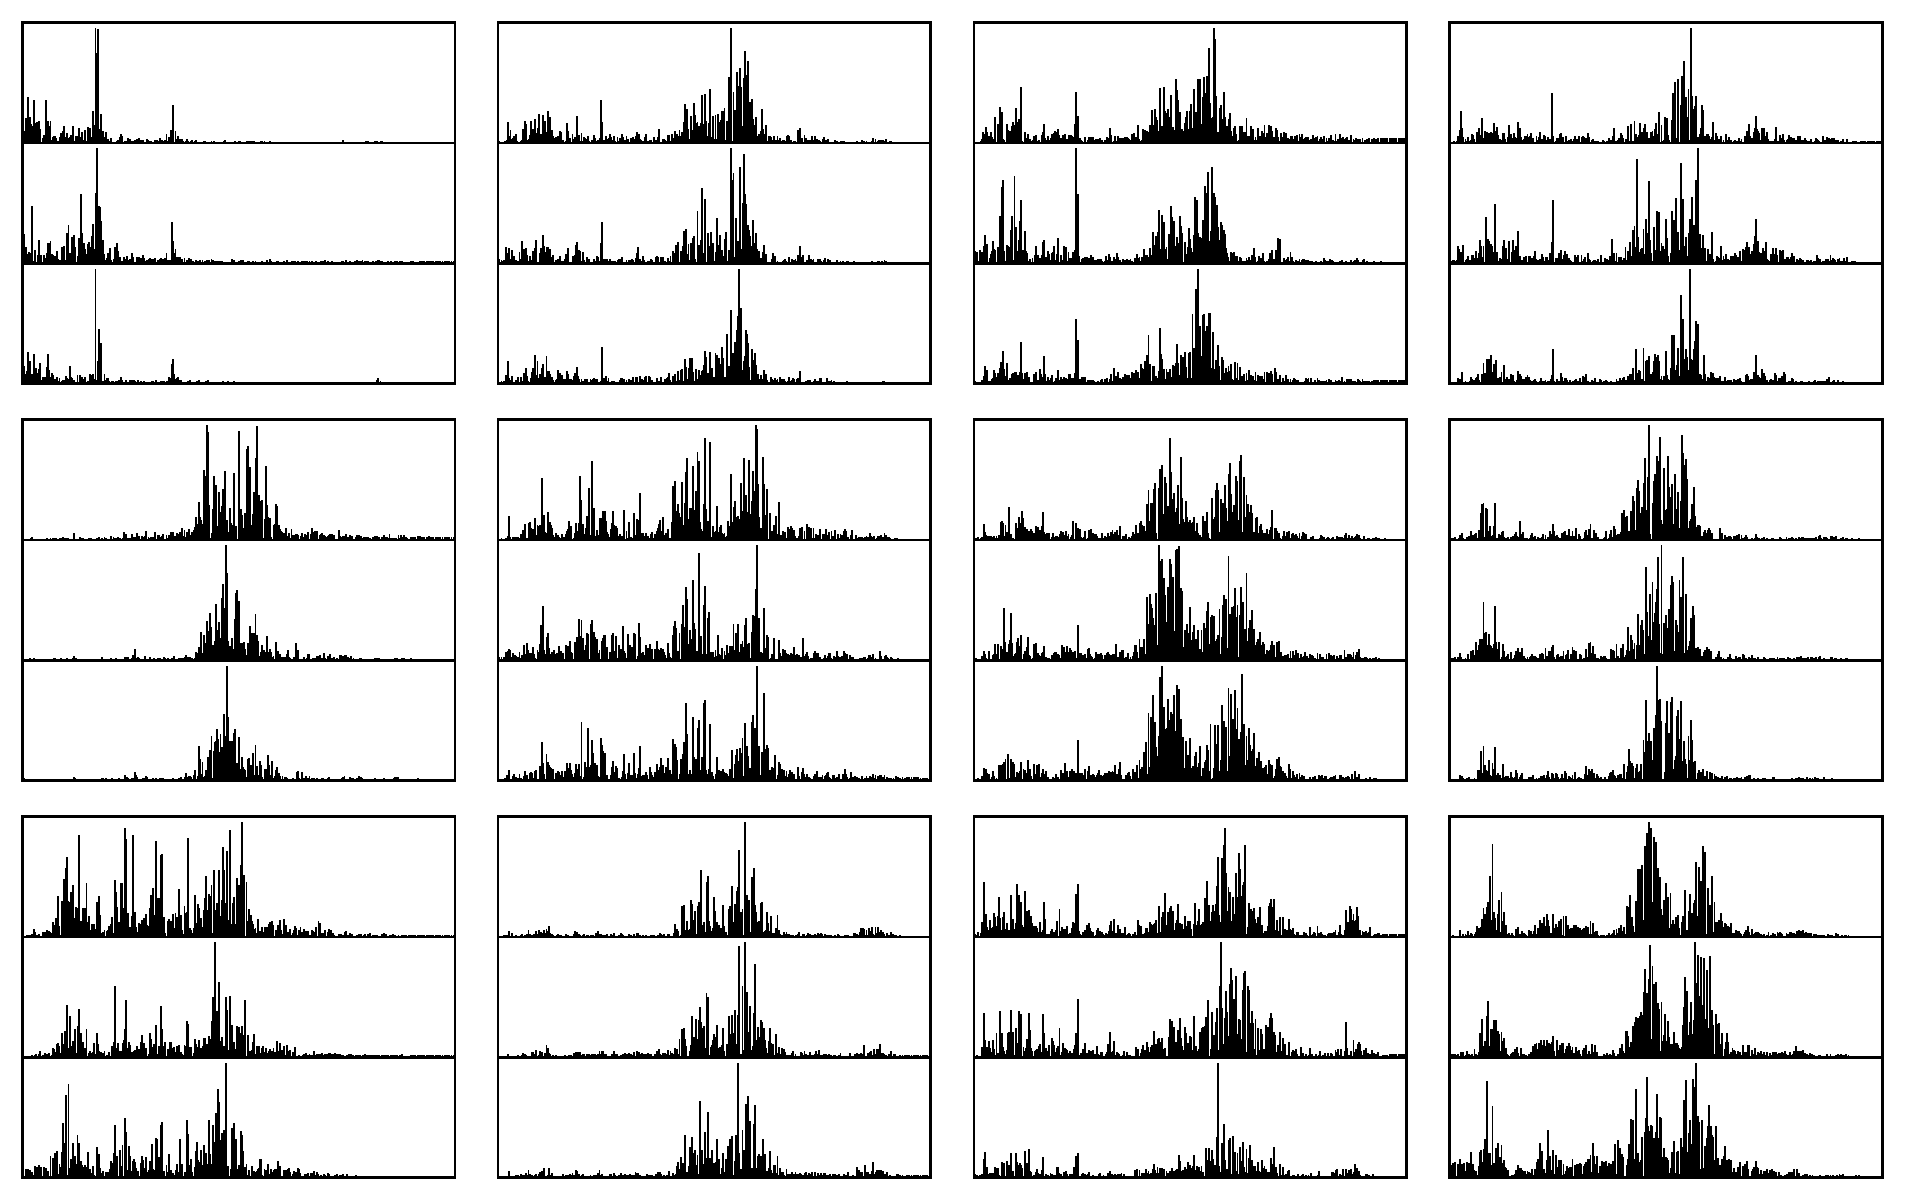
\includegraphics[height=8cm]{rdft}
  \caption{12类信号RDFT频谱序列}
  \label{fig:rdft}
\end{figure}

从图~\ref{fig:rdft}中可以看出,经过RDFT的预处理之后,获得的信号频谱序列
的类内相似性和类间区分性比图~\ref{fig:series}显示的时域信号片段更高。

在特征提取阶段,可以改变下采样操作的核宽度,从而得到具有不同维度$L$的特
征。选择适当的特征维度L也是影响模型诊断效果的一个关键因素。如果$L$值过大,
那么下采样在特征提取过程中起到的作用就相对比较微弱,无法过滤掉信号中特定
频段的一些噪声,同时过大的特征维度也会减慢分类器的训练和预测速度;相反,
如果$L$值过小,那么最终提取的特征向量将会丢失原始信号片段中的过多信息,从
而导致分类器预测效果变差。分别取特征个数$L$为3、6、12、24、48、96、192、
384(对应于下采样操作的核宽度分别为128、64、32、16、8、4、2、1)的情况下,
使用表~\ref{tab:classifier_desc}中列出的训练数据单独训练级联SVM分类模型中
的5个子分类器。表~\ref{tab:dim_performance}列出了级联分类模型在测试集上的
平均精确度、平均召回率和平均F1-Score等评价指标。
\begin{table}[htb]
  \centering
  \begin{minipage}[t]{0.8\linewidth}
  \caption{不同特征个数下级联分类模型的诊断效果}
  \label{tab:dim_performance}
    \begin{tabularx}{\linewidth}{XXXX}
      \toprule[1.5pt]
        特征个数 & 平均精确率 & 平均召回率 & 平均F1-Score \\
      \midrule[1pt]
        3   & 0.7549 & 0.6676 & 0.6615 \\
        6   & 0.8153 & 0.7963 & 0.7659 \\
        12  & 0.8313 & 0.8526 & 0.8318 \\
        24  & 0.9123 & 0.8950 & 0.8913 \\
        48* & 0.9195 & 0.9173 & 0.9167 \\
        96  & 0.9117 & 0.9050 & 0.9057 \\
        192 & 0.9174 & 0.9031 & 0.9032 \\
        384 & 0.9125 & 0.8998 & 0.8939 \\
      \bottomrule[1.5pt]
    \end{tabularx}
  \end{minipage}
\end{table}

级联分类模型在测试集上的预测精度随特征个数的变化趋势如图~\ref{fig:dim_acc}
所示。
\begin{figure}[ht]
  \centering
  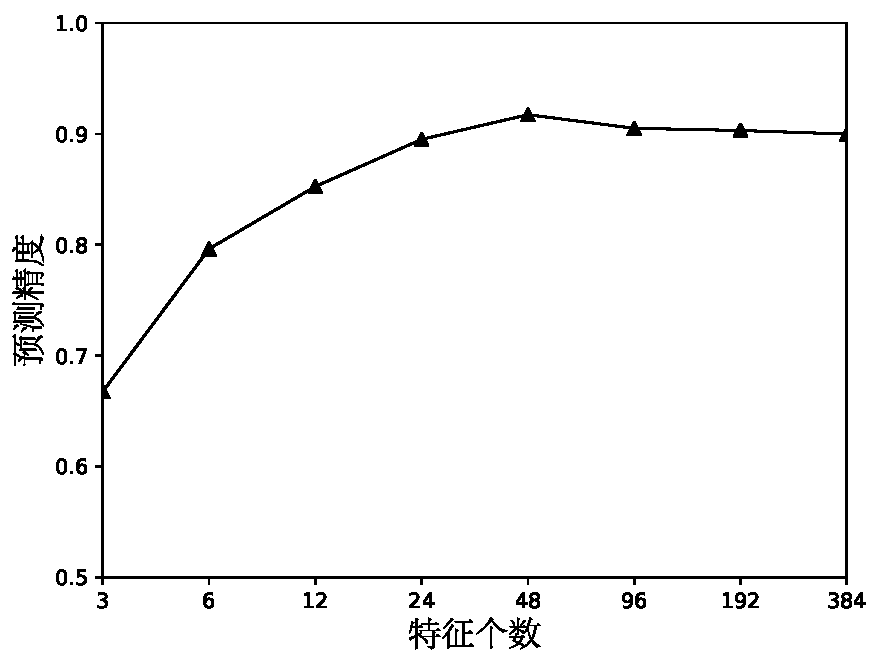
\includegraphics[height=7cm]{dim_acc}
  \caption{预测精度特征个数的变化趋势}
  \label{fig:dim_acc}
\end{figure}

可以看出,模型在特征个数取48时,模型的预测精度达到最高,为91.73\%。因此可
以将$L=48$作为最终的选择。表\ref{tab:chap2:classification_report}给出了此
时模型在测试集上各类的精确率、召回率、F1-Score等评价指标。
\begin{table}[htb]
  \centering
  \begin{minipage}[t]{0.8\linewidth} % 如果想在表格中使用脚注,minipage是个不错的办法
  \caption{基于级联SVM的故障诊断模型在测试集上的评估情况}
  \label{tab:chap2:classification_report}
    \begin{tabularx}{\linewidth}{XXXXX}
      \toprule[1.5pt]
        故障类型    & 精确率 & 召回率 & F1-Score \\
      \midrule[1pt]
        正常        & 1.0000 & 1.0000 & 1.0000 \\
        钢球, 0.007 & 0.6578 & 0.8366 & 0.7365 \\
        钢球, 0.014 & 0.7980 & 0.7207 & 0.7574 \\
        钢球, 0.021 & 0.7546 & 0.6268 & 0.6848 \\
        钢球, 0.028 & 1.0000 & 1.0000 & 1.0000 \\
        内圈, 0.007 & 0.8920 & 0.9846 & 0.9360 \\
        内圈, 0.014 & 0.9490 & 0.9503 & 0.9496 \\
        内圈, 0.021 & 0.9703 & 0.9962 & 0.9831 \\
        内圈, 0.028 & 1.0000 & 1.0000 & 1.0000 \\
        外圈, 0.007 & 0.9859 & 0.9809 & 0.9834 \\
        外圈, 0.014 & 0.9935 & 0.9796 & 0.9865 \\
        外圈, 0.021 & 0.9274 & 0.8426 & 0.8830 \\
      \midrule[1pt]
        平均(总计)& 0.9195 & 0.9173 & 0.9167 \\
      \bottomrule[1.5pt]
    \end{tabularx}
  \end{minipage}
\end{table}

从表~\ref{tab:chap2:classification_report}可以看出,正常状态、钢球部位0.028
英寸故障、内圈部位0.028英寸故障的测试样本的预测结果与样本的真实标签完全一致,
其他故障类型的样本或多或少都存在预测结果错误的情况,尤其是钢球部位0.007英寸、
0.014英寸、0.021英寸的三类故障样本,本章的模型预测效果较差,F1-Score分别只有
73.65\%、75.74\%、68.48\%。

图~\ref{fig:series}中展示的$12\times 3$个信号频谱序列经过核宽度$F=8$的平均值
下采样操作后,获得的长度$L=48$的特征向量如图~\ref{fig:average_pooling_features}
所示。
\begin{figure}[ht]
  \centering
  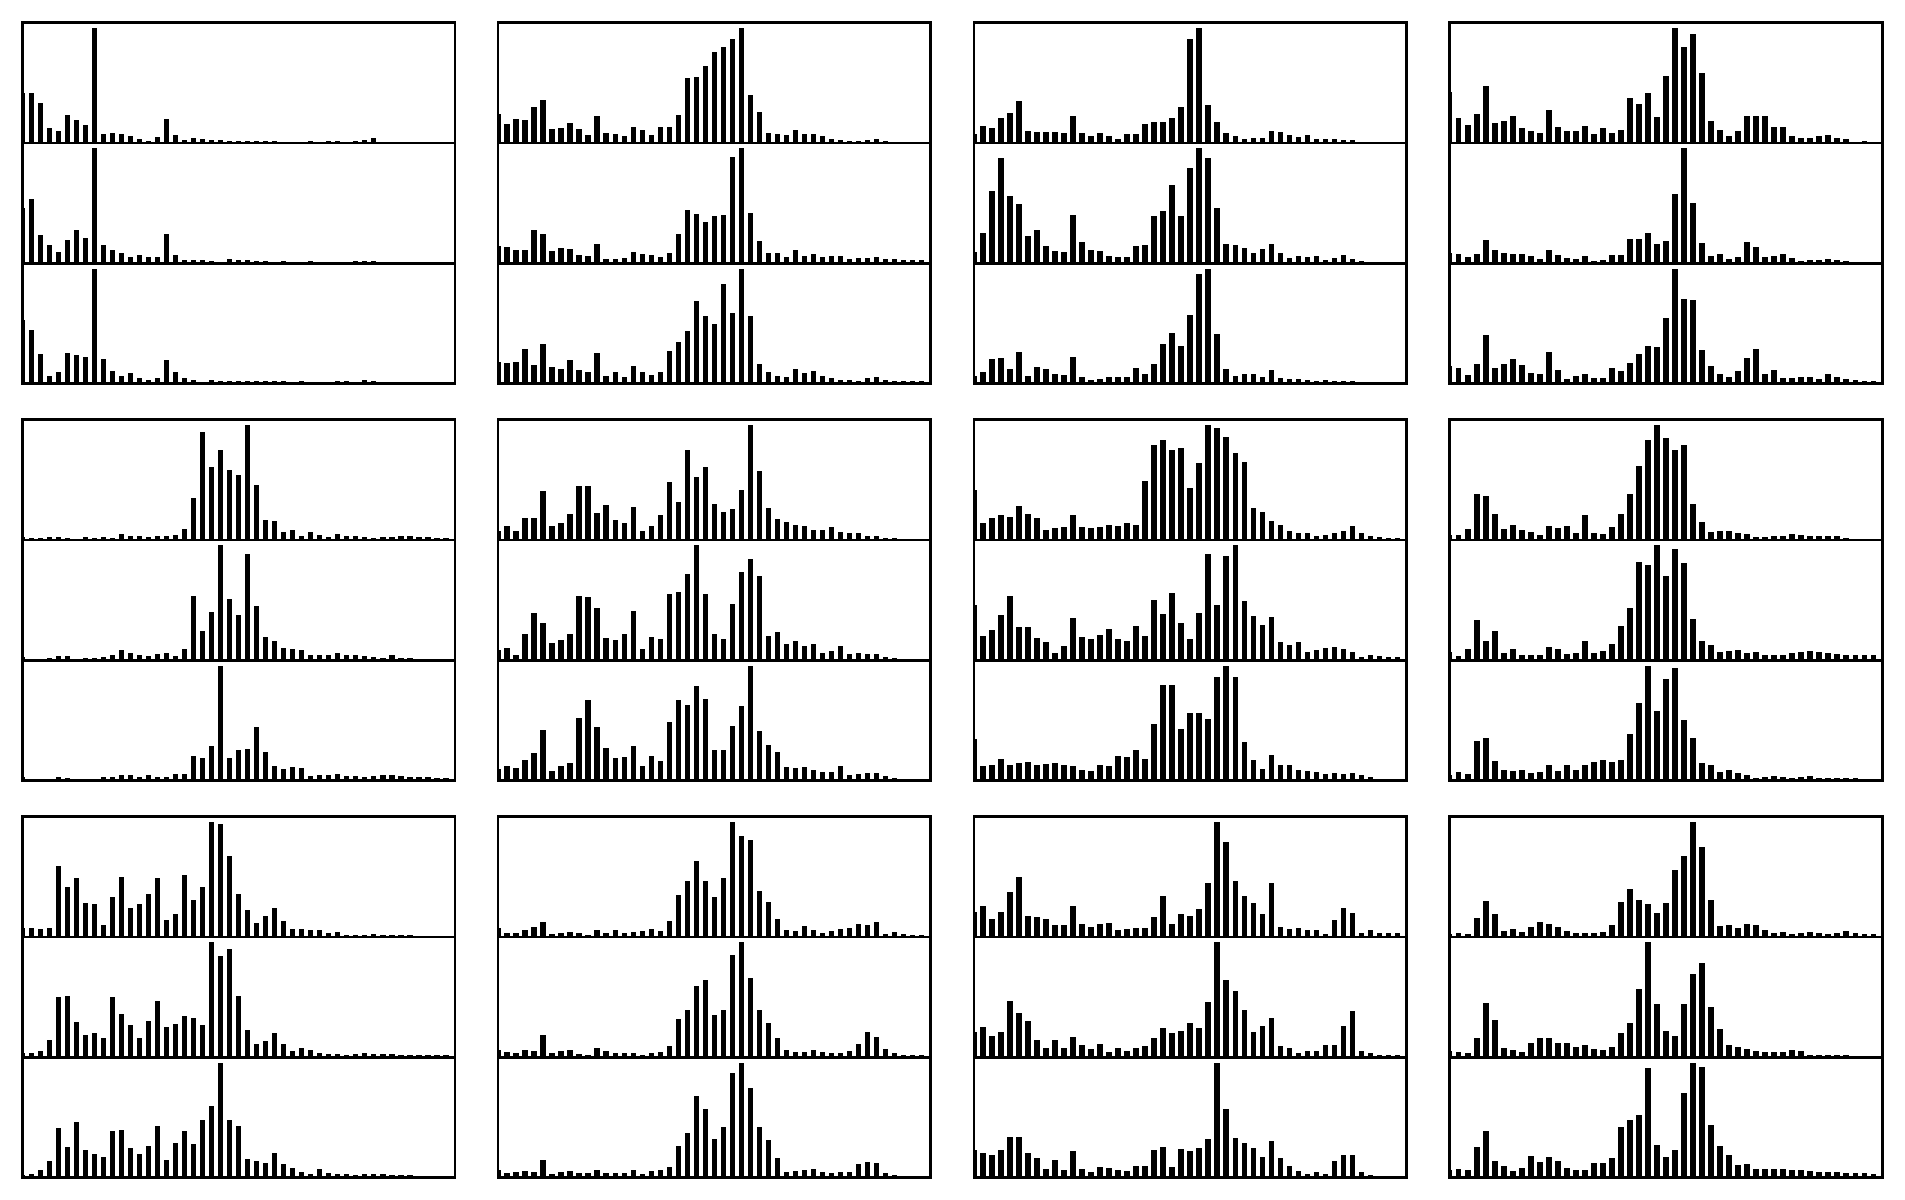
\includegraphics[height=8cm]{average_pooling_features}
  \caption{基于RDFT和平均值下采样提取的特征向量}
  \label{fig:average_pooling_features}
\end{figure}

可以看出,与图~\ref{fig:rdft}中显示的RDFT信号频谱序列相比,使用本章中的特征提
取方法获得的特征向量的类内相似性和类间区分性更高。

\section{小结}

本章介绍了信号处理中经常用到的实数形式的傅立叶变换,以及传统的机器学习算法中经典的
支持向量机算法。之后详细介绍了本章中设计的基于单一尺度的故障特征提取方法和基于
支持向量机算法的级联诊断模型。特征提取阶段使用了平均值下采样来对信号频谱序列
的特征个数进行压缩,同时也能够减弱信号中特定频谱的噪声对诊断效果的影响。另外,由于
可以通过改变下采样的核宽度来控制特征向量的维度,从而能够得到不同尺度下的特征,因此本文
通过对比实验考察了不同尺度的特征对诊断模型的影响,得出在特征维度为48时,模型
预测精度达到最高,为91.73\%。此外也通过精确率、召回率、F1-Score等指标对模型在
测试集上的预测效果进行评估,发现在某些类别的样本上表现并不理想,这也是后面的章
节中设计的模型需要进一步提升的地方。
